\chapter{Numerical Results}

In this chapter the main calculations of the proposed theories and will be presented.

\section{Verification}

\section{Validation of a One-step $\theta$ scheme}
The numerical benchmark presented in \cite{Hron2006} has been chosen for validation of the \textit{One-step $\theta$} scheme presented in chapter. The benchmark has been widely accepted throughout the fluid-structure interaction community as a rigid validation benchmark. This is mainly due to the diversity of tests included, challenging all the main components of a fluid-structure interaction scheme. \\
The computational domain is based on the \textit{von Kármán vortex street}, where a cylinder is intentionally placed off center in a pipe. This configuration initiates a periodic shedding of vortices, as some fluid moves past the cylinder. In \cite{Hron2006}, an elastic flag is placed behind the cylinder. \\

\begin{figure}
  \centering
    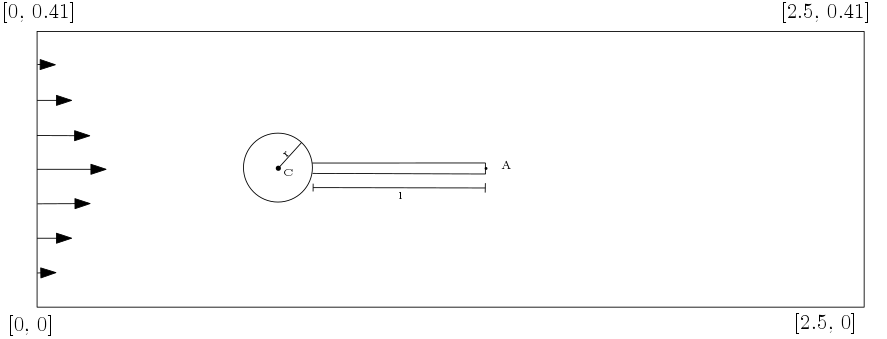
\includegraphics[scale=0.5]{./Fig/turekflag.png}
      \caption{Computational domain of the validation benchmark}
\end{figure}
\newpage
The benchmark is divided into three main test environments.
In the first environment the fluid solver is tested for a range of different inflow parameters. \\
The second environment regards the structure implementation, regarding bending of the elastic flag. In this thesis the third and final environment will be evaluated, testing a full fluid-structure interaction problem. 



\ 
The others have been tested and proved to be an essential part of the development of the solver, but will for brevity not be reported. \\ \\

The fluid-structure interaction validation benchmark is divided into three different problems with increasing difficulty, posing different challenges to the implementation.
Each problem alters the fluid and solid parameters to provoke different behavior of the system.

\subsection{Boundary and Initial Conditions}
A parabolic velocity profile on the form,
\begin{align*}
v_f(0, y) = 1.5 U\frac{(H -y)y}{(\frac{H}{2})^2} 
\end{align*}
is set on the left channel inflow. H is the height of the channel, while the parameter U is set differently to each problem to induce different flow profiles. \
At the right channel outflow, the pressure is set to $p = 0$. \
No-slip boundary conditions are enforced on the channel walls, and on the whole inner geometry consisting of the circle and the elastic flag. A 

Several quantites for comparion is presented in \cite{Hron2006} for validation purposes. We will report
\begin{itemize}
\item The position of point A(t) as the strucutre undergoes deformation.
\item Drag and lift forces exerted on of the whole interior geometry in contact with the fluid, consisting of the rigid circle and the elastic beam.
\begin{align*}
(F_D, F_L) = \int_{\Gamma} \mathbf{\sigma} \cdot \mathbf{n} dS
\end{align*}
Where \textbf{n} is the unit normal vector, pointing into the fluid domain.
\end{itemize}
The amplitude and mean values for the time dependent properties are calculated from the last period of oscillations, together with the period.

\begin{table}[h]
\centering
\caption{Benchmark environment}
\label{my-label}
\begin{tabular}{ |p{3cm}||p{2cm}|p{2cm}|p{2cm}|  }
 \hline
 \multicolumn{4}{|c|}{Solid parameters} \\
 \hline
 parameter              & FSI1 & FSI2 & FSI3 \\
 \hline
 $\rho^s [10^{3} \frac{kg}{m^3}]$ & 1    & 10   & 1    \\
$\nu^s$ & 0.4  & 0.4  & 0.4  \\
$\mu^s  [10^{6}\frac{kg}{ms^2}]$  & 0.5  & 0.5  & 2.0  \\
 \hline
 \multicolumn{4}{|c|}{Fluid parameters} \\
 \hline
$\rho^f [10^{3}\frac{kg}{m^3}]$ & 1    & 1    & 1    \\
$\nu^f  [10^{-3}\frac{m^2}{s}]$  & 1    & 1    & 1    \\
U                      & 0.2  & 1    & 2    \\
parameter              & FSI1 & FSI2 & FSI3 \\
Re                     & 20   & 100  & 200 \\
\hline
\end{tabular}
\end{table}


\subsection{FSI1}
The first environment yields a steady state solution for the system, inducing small deformations to the elastic flag. However, due to the small deformations of order $10^{-6}$, FSI1 doesn't provide a rigorous test of the choice of mesh extrapolation model. In our studies, the mesh extrapolation model was omitted, still obtaining reasonable results. This proves that the FSI validation case can be misguiding, in terms of validating the mesh extrapolation model. 
 

\subsection{FSI2}
The second environment results in a periodic solution. The inflow parameter .
It proved to be one of the most demanding tests due to its large deformation, leading to the risk of entangled mesh cells. Therefore a high quality extrapolation of the solid deformation into the fluid is needed. 
\\
\subsection{FSI3}
The final environment does not induce deformation to the extent of the FSI2 benchmark. However a critical phase in the transition to the periodic solution was discovered, where the pressure oscillation induces a large deformation to the system.
\begin{table}[h!]
\centering
\caption{FSI 3 - Laplace}
\label{my-label}
\begin{tabular}{ |p{1cm}||p{1cm}|p{2.5cm}|p{2.5cm}|p{2.7cm}|p{2.7cm}|p{1.2cm}|}
 \hline
  \multicolumn{6}{|c|}{$\Delta t = 0.01 \theta = 0.51$} \\
   \hline
nel & ndof & ux of A [x $10^{3}$]  &uy of A [x $10^{3}$]& Drag  & Lift \\
 \hline
1216 &5797& $-1.79 \pm  1.80$  & 3.29 $\pm$  26.48 & 439.35  $\pm$  12.04 &  1.96 $\pm$  142.30 \\
2295 &10730& -2.48 $\pm$  2.48 &1.64 $\pm$  32.84   & 449.76   $\pm$  18.01 &  3.40  $\pm$  153.47\\
5963 &27486 & -2.47   $\pm$  2.45 &1.27 $\pm$  32.89 & 456.59  $\pm$  18.73 &  -1.55  $\pm$  153.46\\
 \hline
  \multicolumn{6}{|c|}{$\Delta t = 0.001 \theta = 0.501$} \\
   \hline
 nel & ndof & ux of A [x $10^{3}$]  &uy of A [x $10^{3}$]& Drag  & Lift \\
1216 &5797& --2.17$\pm$  2.08 &     3.32     $\pm$  29.07 &439.98 $\pm$  14.08  &  1.91 $\pm$  151.71\\
2295 &10730& -3.04 $\pm$  2.88 &  1.51  $\pm$  35.88 & 452.04  $\pm$  22.41 &  3.30      $\pm$  160.11 \\
5963 &27486 & -3.03$\pm$  2.85 &  1.23 $\pm$  35.97  & 459.45  $\pm$  23.80 &  1.53  $\pm$  160.14 \\
\hline
\multicolumn{6}{|c|}{$\Delta t = 0.001 \theta = 0.5$} \\
   \hline
 nel & ndof & ux of A [x $10^{3}$]  &uy of A [x $10^{3}$]& Drag  & Lift \\
\hline
1216 &5797& -2.17  $\pm$   2.08 &  3.32 $\pm$   29.08  & 439.99  $\pm$   14.08  & 1.90 $\pm$  151.72 \\
2295 &10730& -3.04 $\pm$  2.88  & 1.51  $\pm$  35.89  & 452.04   $\pm$  22.41 &  3.30 $\pm$  160.12 \\
\hline
\end{tabular}
\end{table}


\begin{table}[h!]
\centering
\caption{FSI 3 - Biharmonic BC1}
\label{my-label}
\begin{tabular}{ |p{1cm}||p{1cm}|p{2.5cm}|p{2.5cm}|p{2.7cm}|p{2.7cm}|p{1.2cm}|}
 \hline
  \multicolumn{6}{|c|}{$\Delta t = 0.01 \theta = 0.51$} \\
   \hline
nel & ndof & ux of A [x $10^{3}$]  &uy of A [x $10^{3}$]& Drag  & Lift \\
 \hline
1216 &5797& -1.77 $\pm$ 1.79  & 3.58 $\pm$  26.21& 439.60  $\pm$ 12.21  &  -1.84  $\pm$  139.29 \\
2295 &10730& -2.43,+/  2.44  & 1.75  $\pm$  32.55 & 449.95     $\pm$  17.95  &  3.74 $\pm$  150.56 \\
5963 &27486 & 1 & 1& 456.91  $\pm$  18.79 &  -1.21  $\pm$   15.17\\
%BAD RES IN DX AND DY
 \hline
  \multicolumn{6}{|c|}{$\Delta t = 0.001 \theta = 0.501$} \\
   \hline
 nel & ndof & ux of A [x $10^{3}$]  &uy of A [x $10^{3}$]& Drag  & Lift \\
 1216 &5797& -3.39$\pm$  3.38 &  1.27 $\pm$  36.66  & 413.03  $\pm$  51.59 & 56.66  $\pm$  222.03 \\
\hline
\multicolumn{6}{|c|}{$\Delta t = 0.001 \theta = 0.5$} \\
   \hline
 nel & ndof & ux of A [x $10^{3}$]  &uy of A [x $10^{3}$]& Drag  & Lift \\
\hline
1216 &5797&--2.18  $\pm$ 2.10 &  3.56   $\pm$  29.04 & 440.24  $\pm$  14.42  & -1.80  $\pm$  150.97\\
\hline
\end{tabular}
\end{table}

\begin{table}[h!]
\centering
\caption{FSI 3 - Biharmonic BC2}
\label{my-label}
\begin{tabular}{ |p{1cm}||p{1cm}|p{2.5cm}|p{2.5cm}|p{2.7cm}|p{2.7cm}|p{1.2cm}|}
 \hline
  \multicolumn{6}{|c|}{$\Delta t = 0.01 \theta = 0.51$} \\
   \hline
nel & ndof & ux of A [x $10^{3}$]  &uy of A [x $10^{3}$]& Drag  & Lift \\
 \hline
1216 &5797& -1.74  $\pm$  1.76 & 3.56 $\pm$  26.01 & 439.41$\pm$ 12.21  & -1.35    $\pm$  138.74\\
2295 &10730 & -2.39   $\pm$  2.40 &  1.76  $\pm$  32.27 & 449.71$\pm$ 18.16 &  3.71   $\pm$  149.97\\
 \hline
  \multicolumn{6}{|c|}{$\Delta t = 0.001 \theta = 0.501$} \\
   \hline
 nel & ndof & ux of A [x $10^{3}$]  &uy of A [x $10^{3}$]& Drag  & Lift \\
 1216 &5797& -3.39   $\pm$  3.38 &   1.23   $\pm$  36.61 &   413.26 $\pm$  51.82  &   57.19  $\pm$  222.65\\
 2295 &10730& -4.70  $\pm$  4.71& 1.49       $\pm$  44.62& 427.91$\pm$  93.17 &  44.38  $\pm$  268.05 \\
\hline
\multicolumn{6}{|c|}{$\Delta t = 0.001 \theta = 0.5$} \\
   \hline
 nel & ndof & ux of A [x $10^{3}$]  &uy of A [x $10^{3}$]& Drag  & Lift \\
\hline
1216 &5797&-2.17$\pm$  2.09 & 3.54  $\pm$  28.95 & 440.13  $\pm$  14.45  &  -1.38  $\pm$  150.96\\
\hline
\end{tabular}
\end{table}


\section{Mesh movement}
The final enviroment
